% !TEX TS-program = pdflatex
% !TEX encoding = UTF-8 Unicode
% !TEX root = Wine_Quality-Presentation.tex
% !TEX spellcheck = en-EN
% !BIB program = biber

\documentclass{beamer}
\usepackage{graphicx}
\usepackage{paralist}

\author{Joshua Paul Barnard}
\title{Predicting Wine Quality by comparing Linear Regression with Machine Learning Techniques.}
\titlegraphic{\vspace{-10mm}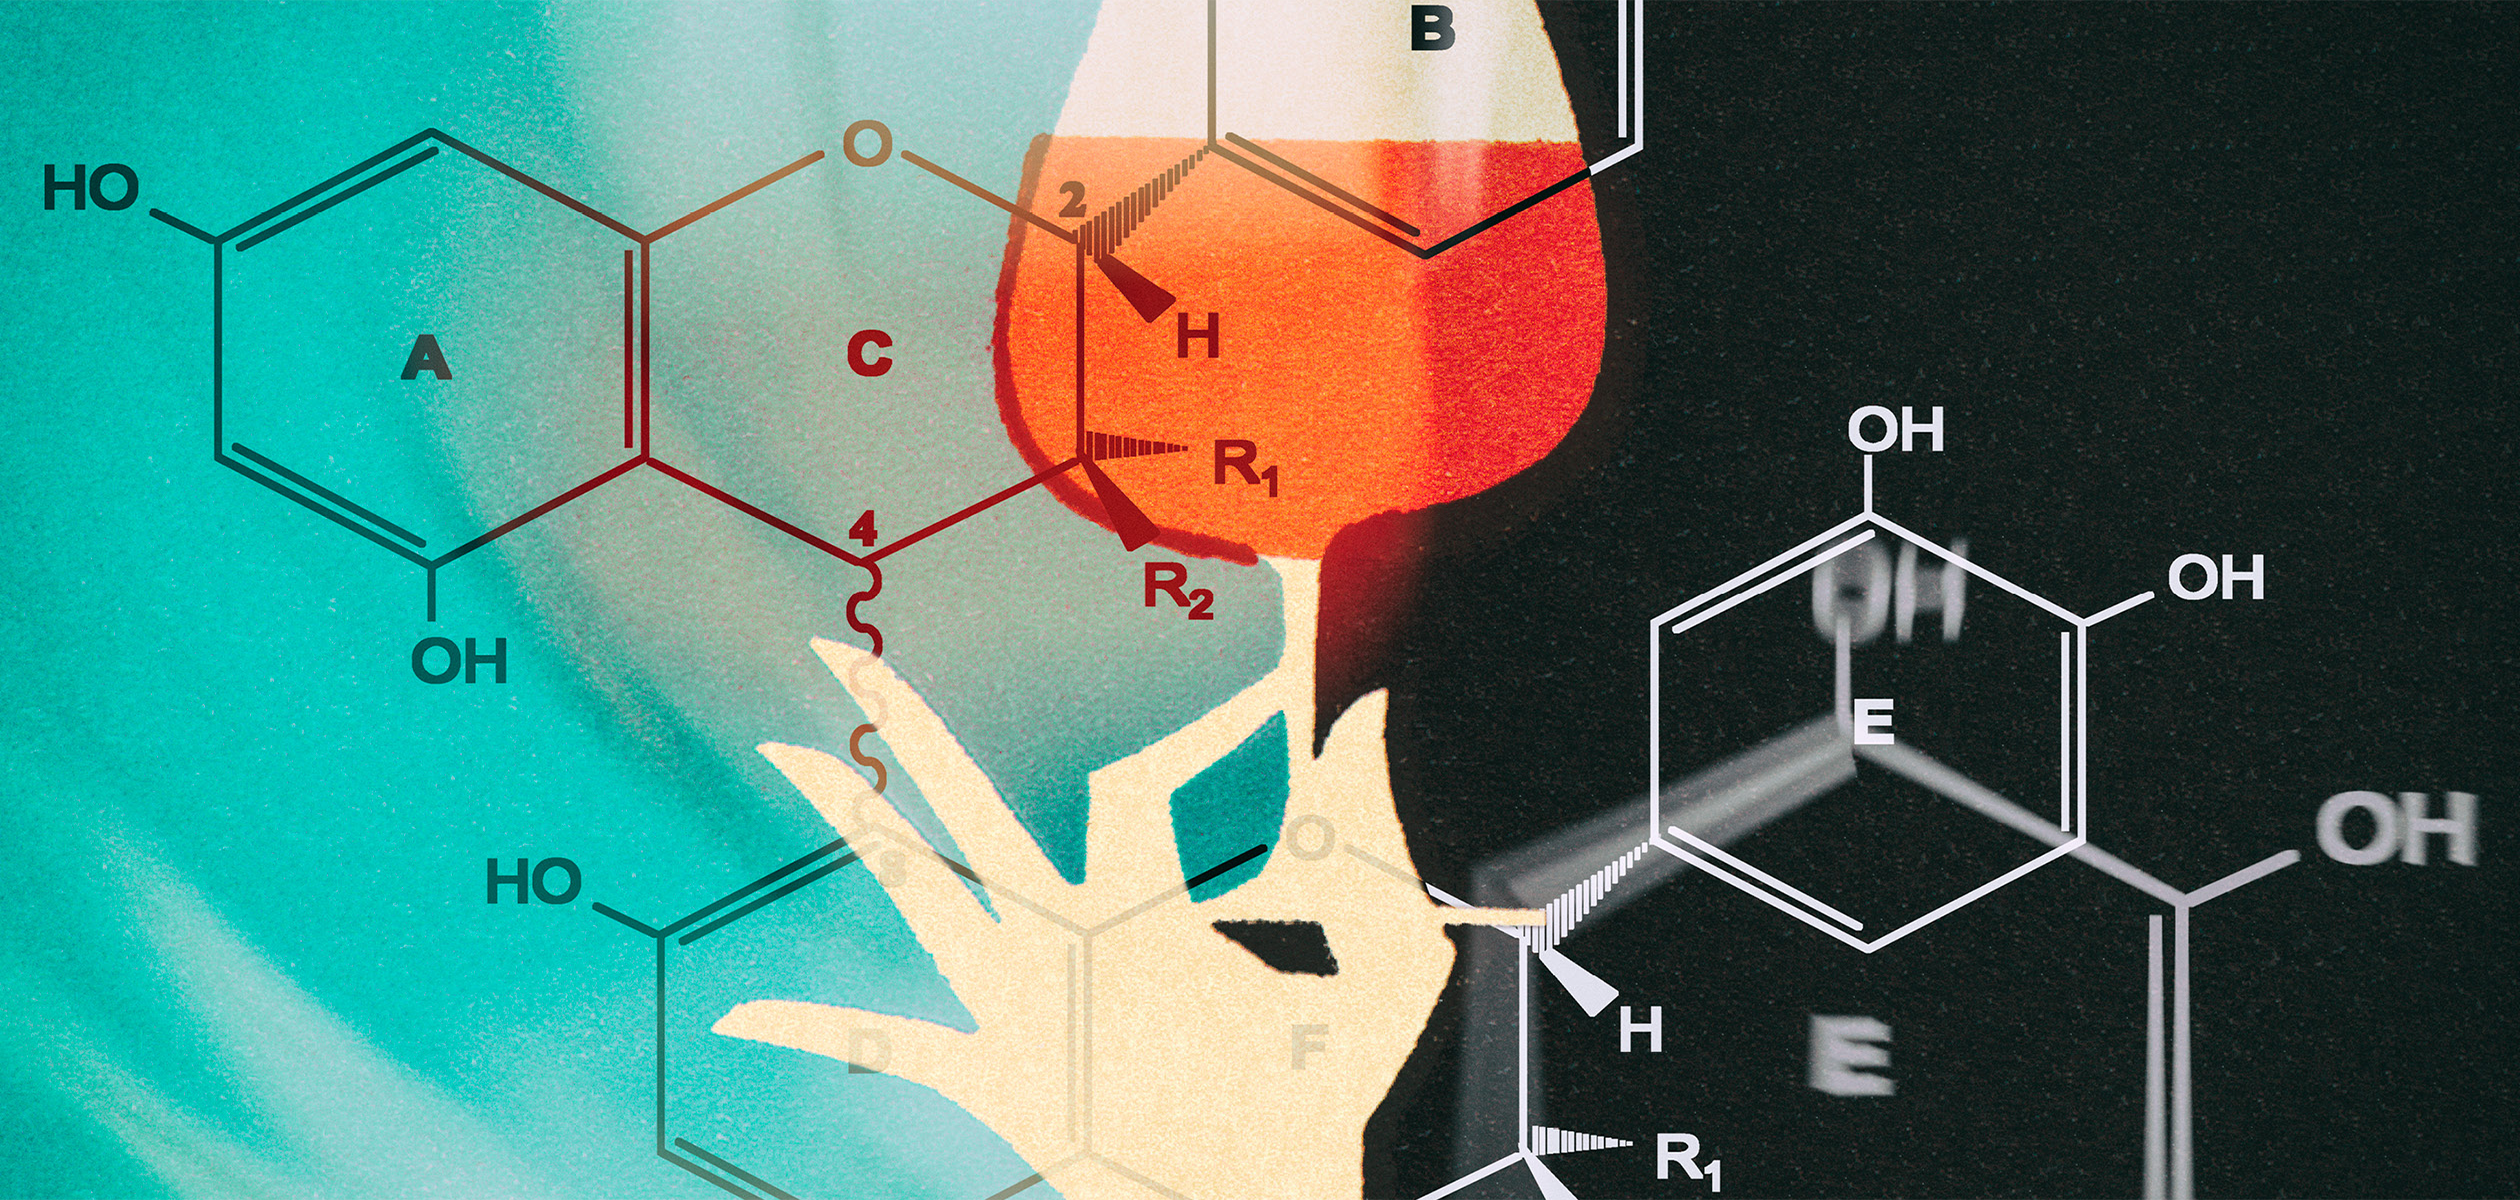
\includegraphics[width = .8\textwidth]{images/wine science.png}} 
\date{\vspace{-5em}} 


\mode <presentation>
\usetheme{Warsaw}
\usecolortheme{default}

\setbeamerfont{footline}{size=\fontsize{5}{8}\selectfont}

\definecolor{darkred}{rgb}{20,0,0}
\definecolor{darkgreen}{RGB}{40,110,20}
\definecolor{darkpurple}{RGB}{30,0,30}
\definecolor{chardonnay}{RGB}{255, 255, 204}

\setbeamercolor*{palette primary}{fg=white, bg=darkgreen}


\begin{document}
	{
		\setbeamertemplate{footline}{} 
		\setbeamertemplate{headline}{} 
		\begin{frame}
			\vspace{-35pt}
			\maketitle
		\end{frame}
	}

	\section{}

	\subsection{What is Wine Quality?}
	\begin{frame}
		\frametitle{What is Wine Quality?}
			\begin{itemize}
				\item The quality of wine is complex and is considered to be difficult to understand, with its quazi-aesthetic character and relationship to personal taste, it is peculiarly hard to pinpoint.  
				\item Some suggest that quality is more objective, with a crucial determinant in the quality of wines to be an absence of faults.  While others suggest that a wines quality is perceived, and is based on its 'fit for a purpose', which brings up more dimensions as to what a purpose even is. 
				\item Due to the concept of wine quality being hard to define precisely, we will focus on the more objective physicochemical properties to determine the quality of wine.
			\end{itemize}
			\begin{center}
				\includegraphics[width = 0.2\textwidth]{images/quality-in-wine.png}
			\end{center}
	\end{frame}


	\subsection{Motivation and Reasoning}
		\begin{frame}
		\frametitle{Motivation and Reasons}
		\begin{columns}
			\column{.6\textwidth}
			
			\begin{itemize}
				\item A winery is a business, and just like any business they need to know which wines are worth distributing and marketing.  Wine quality can be used as a metric to help determine the marketability of one wine to another.  
				\item Understanding which chemical are responsible for a wine's quality allows for winemakers to add and remove wanted and unwanted chemicals from their wine wines while maintaining quality.
			\end{itemize}
			
			\column{.5\textwidth}
			
			\includegraphics[width=\textwidth]{images/tuscan wine.png}
		\end{columns}
	\end{frame}

	
	\section{ETL (Extract, Transform, Load)}
	
	\subsection{About the Data}
	
	\begin{frame}
		\frametitle{The Source of our Data}

		\begin{columns}
			

			
			\column{.5\textwidth}
								\includegraphics[width=0.3\textwidth]{images/paulo cortez headshot.jpg}
								
								Paulo Cortez \par
								\begin{footnotesize}
								Department of Information Systems | School of Engineering | University of Minho, Portugal \par
	% make an empty space here
									P. Cortez, A. Cerdeira, F. Almeida, T. Matos and J. Reis. Modeling wine preferences by data mining from physicochemical properties. In Decision Support Systems, Elsevier, 47(4):547-553, 2009.
								\end{footnotesize}
				
			\column{.5\textwidth}
						\vspace{-15pt}
				\begin{itemize}
					\item Two datasets are related to red and white variants of the "Vinho Verde" wine from the north of Portugal.
					\item Vinho verde is a unique product from the Minho (northwest) region of Portugal. Medium in alcohol, is it particularly appreciated due to its freshness (specially in the summer). More details can be found at: http://www.vinhoverde.pt/en/ 
				\end{itemize}
		\end{columns}
	\end{frame}

	
	\subsection{Extracting the Data}
	\begin{frame}
		\frametitle{The source data}
		\begin{itemize}
		\item Our data came from two separate datasets, one for white wines and one for red wines.
		\item Both were saved as .csv, yet the delimiter was a semicolon and not a comma.
		\end{itemize}  
		\includegraphics[width=\textwidth]{images/loading datasets.png}
		\begin{itemize}
		\item The White Wine Dataset contains 4898 samples. 
		\item The Red Wine Dataset contains 1599 samples. 
		\item Combined we have 6497 total samples.
		\end{itemize}
	
	\end{frame}

	
	\begin{frame}
		\frametitle{Merging the datasets and creating indicator variables}
		\begin{itemize}
			\item We then created 3 new variables in the two separate datasets:  
			wine\_type - is a string variable containing: 'Red Wine' or 'White Wine' 
			\item Red\_Wine - is an indicator (dummy) variable to allow us to use the category in our regression analysis.  1 indicates Red Wine, and 0 indicates White Wine.  
			\item White\_Wine - is an indicator (dummy) variable to allow us to use the category in our regression analysis.  1 indicates White Wine, and 0 indicates Red Wine.  
		\end{itemize}
			\begin{center}
				\includegraphics[width=.3\textwidth]{images/wine_type.png}
			\end{center}
	\end{frame}

	
	\subsection{Transformations}
	\begin{frame}
		\frametitle{What transformations were tried}
		During the modeling stage we noticed some issues with the residuals for the Quality and Alcohol variables.  \par
		\vspace{10pt}
		We tried various transformations, including:  
		\begin{itemize}
			\item Log Transformations (base: 2, e, and 10)
			\item Power Transformations (2, 3, and 4)
			\item Root Transformations (2, 3, and 4)
			\item Inverse Transformations
			\item Reciprocal Transformations
			\item Centering and Scaling Transformations (standardization)
		\end{itemize}
	\vspace{10pt}
			Various transformations were attempted, but they did not help.  \par
	\end{frame}

	\subsection{Loading into SQL Database}
	
		\begin{frame}
			\frametitle{SQL Database}
				\begin{columns}
					\column{.5\textwidth}
						\begin{itemize}
							\item We created the architecture for our SQL database.
							\item The database includes all of our original variables, plus our new categorical variable and its 2 indicator variables.
							\item We then loaded our dataset into our new database using sqlite3.
						\end{itemize}
					
					\column{.5\textwidth}
						\includegraphics[height=.85\textheight]{images/sql.png}
				\end{columns}

		
		\end{frame}
	
	
	\section{EDA (Exploratory Data Analysis)}
	
		\subsection{Domain Knowledge}
			\begin{frame}
				\frametitle{About the Variables}
					\begin{itemize}
						\begin{footnotesize}
						\item \textbf{Quality:}  Is the median of at least 3 evaluations made by wine experts, with each expert grading the wine quality from 0 to 10, with 0 representing 'very bad' and 10 indicating 'very excellent' 
						
						\item \textbf{Wine Type:}  People have preferences for different the types/colours of wine, which can influence a judge's expectations and perception of quality.  
						
						\item \textbf{Fixed Acidity:}  Usually refers to the amount of non-acetic acids in a wine.  In this dataset is refers to the concentration of Tartaric Acid. 
						
						\item \textbf{Volatile Acidity:} The amount of acetic acid in a wine.  VA is vinegar, and if levels are too high it can lead to an unpleasant, vinegar taste.  A measure of volatile acidity is used routinely as a indicator of wine spoilage.  \par 
						A taster's sensitivity to acetic acid will vary, but most people can detect excessive amounts at around 600 mg/L.  
						
						\item \textbf{Citric Acid:} Can add ‘freshness’ and flavor to wines.  One of the three primary acids found in wine grapes, along with tartaric, and malic.			
						
						\item \textbf{Residual Sugar:} A mixture of glucose and fructose, it is the amount of sugar remaining after fermentation stops, wines are typically between 1 gram/liter and 45 grams/liter. 
						\end{footnotesize}
					\end{itemize}
			\end{frame}
	
	
	\begin{frame}
	\frametitle{About the Variables}
	\begin{itemize}
		\begin{footnotesize}			
			\item \textbf{Chlorides:} Sodium Chloride, the amount of salt in the wine.  People typically do not enjoy salty wines.  
			
			\item \textbf{Free Sulfur Dioxide:} Free form of SO2, helps prevent microbial growth and the oxidation (spoilage) of wine.  Free SO2 is unnoticeable until 50ppm when it imparts a chemically aroma and taste in the wine.  
			
			\item \textbf{Total Sulfur Dioxide:} The amount of free and bound forms of S02.  High concentrations can be an indication of wine faults.  
			
			\item \textbf{Sulphates:} Potassium Sulphate, a wine additive which can contribute to sulfur dioxide (S02) levels.  Has a bitter, salty taste.   
			
			\item \textbf{Density:} The density of wine is close to that of water depending, with dense wines being thick and syrupy.
			
			\item \textbf{pH:} A scale from 0 (very acidic) to 14 (very basic); most wines are between 3-4 on the pH scale.  White Wines are usually more acidic from 3.0 and 3.4.  Red Wines are usually less acidic, from 3.3 and 3.6.
			
 			\item \textbf{Alcohol:} The percent alcohol content of the wine.  Alcohol helps bring out the aromas and tastes in a wine, so it will be more apparent if a wine is of poor quality if it has a higher alcohol content.  Conversely, a good quality wine will be more pleasant and enjoyable with higher alcohol.
		\end{footnotesize}
	\end{itemize}
\end{frame}
	

	\begin{frame}
		\frametitle{Causal Loop Diagram}
			\includegraphics[height=.85\textheight]{images/CLD - Interactions.png}
	\end{frame}
	
	\subsection{Exploring the Dataset}
		\begin{frame}
		\frametitle{ Checking for Unreasonably Low or High Values }
			All of the variables look appropriate, with none of them have a minimum or maximum values outside their expected ranges.  \par
			\vspace{25pt}
		\includegraphics[width=\textwidth]{images/descriptive stats.png}
	\end{frame}
	
	
	\subsection{Variable Analysis}
	\begin{frame}
		\frametitle{ Analyzing our Variables }
			\begin{columns}
				\column{.5\textwidth}
				Highest Correlated Variables with Quality:
				\begin{itemize}
					\item Alcohol:  0.45
					\item Density:  -0.32
					\item Chlorides:  -0.30
					\item Volatile Acidity:  -0.26
				\end{itemize}
			Lowest Correlated Variables with Quality:
			\begin{itemize}
				\item Total Sulfur Dioxide:  -0.055
				\item pH:  0.032
				\item Sulphates:  0.030
				\item Residual Sugar:  -0.017
			\end{itemize}
				\column{.5\textwidth}
				\includegraphics[height=.45\textheight]{images/alcohol vs quality.png} 
				\includegraphics[height=.45\textheight]{images/VA vs quality.png} 
			\end{columns}
		
	\end{frame}
	
	\subsection{Checking for Outliers and Multicollinearity}
	\begin{frame}
		\frametitle{Check for Multicollinearity}
			\begin{footnotesize}
			\begin{columns}
				\hspace{5pt}
				\column{.85\textwidth}
			Based on our Domain Knowledge there might be multicollinearity between the following variables:  \par
			\begin{itemize}
			\item Total Sulfur Dioxide with Free Sulfur Dioxide and Sulphate.  

			\item pH with fixed acidity, volatile acidity, citric acid, total sulfur dioxide, free sulfur dioxide, and sulphates.  

			\item Density with every other variable except quality, Red Wine and White Wine.   
			\end{itemize}
			The following variables had correlations above 0.5 (or less than -0.5):  \par
			\begin{itemize}
			\item Total Sulfur Dioxide and Free Sulfur Dioxide:  0.72
			\item Density and Alcohol:  -0.69 
			\item Density and Residual Sugar:  0.55 
			\end{itemize}
		These correlations make sense based on our domain knowledge, and are not high enough to prevent us from getting good estimates of our coefficients.  
		\vspace{-5pt}
		\column{0.3\textwidth}
		\begin{center}
			Total Sulfur Dioxide:
					\includegraphics[height=.1\textheight]{images/SO2.png}  \par
					pH: \par
					\includegraphics[height=.23\textheight]{images/acidity.png}  \par
					Density: \par
					\includegraphics[height=.35\textheight]{images/density.png}
		\end{center}
			\end{columns}
					\end{footnotesize}
	\end{frame}
	
	
	\begin{frame}
		\frametitle{Check for Outliers}
		To check for outliers we will examine points which are below Q1 - 1.5 x IQR and above Q3 + 1.5 x IQR.  \par
		Based on our EDA we expect potential outliers to exist for:  volatile acidity, citric acid, chlorides, free sulfur dioxide, total sulfur dioxide, sulphates, density.  
		\begin{center}
		\includegraphics[height=.35\textheight]{images/outliers.png}
		\end{center}
		We kept all of the outliers as they were within reason, and carelessly ignoring outliers can lead to fragile models which lack robustness.
	\end{frame}
	
	
	\section{The Models}
	
	\subsection{The Null Model}
	\begin{frame}
		\frametitle{The Null Model}
		\begin{small}
			\begin{columns}
				\column{.7\textwidth}
				
				\begin{itemize}
					\item Quality appears normally distributed.
					\item Quality is integers from 0 to 10, which is ordinal data with each grade being a different rank.  As quality is not a concrete concept, we will treat quality as if it were continuous and interpret the results as more of a percent from 0 to 100.
					\item The Null Model:
					\begin{itemize}
						\item Mean: 5.82 (58.2\%)
						\item Standard Deviation: 0.87
						\item Which gives us a 95 percent chance for a score to fall between 4.1 and 7.5
					\end{itemize}
					\item When comparing the null model with sampled data, our prediction is off by 0.97 on average.
				\end{itemize}
				
				\column{.5\textwidth}
				
				\includegraphics[width=\textwidth]{images/quality histogram.png}
			\end{columns}
		\end{small}
	\end{frame}
	
	\subsection{Linear Regression}
	\begin{frame}
		\frametitle{What is Linear Regression?}
		\begin{itemize}
			\item Linear Regression can be described as:  
		\end{itemize}
		\begin{center}
			\emph{y} = $\beta$$_{0}$ + $\beta$$_{1}$\emph{x}$_{1}$ + ... + $\beta$$_{n}$\emph{x}$_{n}$ $\epsilon$ ,   \par
			$\epsilon$ $\sim$ \emph{N}(0, $\sigma$)   \par
		\end{center}
	\begin{itemize}
		\item Bootstrapping is where we resample from our data, for each sample, and calculate new values for the outcomes and parameters, estimate their distribution and get a better idea of the uncertainty associated with our model.  This allows us to create 95\% Bayesian Credible Intervals and satisfy the OLS assumption of normally distributed errors. 
		\item N-Fold Cross Validation borrows from the idea of bootstrapping to divide the data into N folds (or sections) and loop over each fold to use it as the test set against each training set.  This will yield N-estimates of MSE.  
	\end{itemize}
	\end{frame}
	
	\begin{frame}
		\frametitle{Our Linear Regression Models}
			Our best models based upon our Domain Knowledge:  \par
			\begin{footnotesize}
			\begin{itemize}
				\item All-in Model:  "quality \~{} Red\_Wine + White\_Wine + fixed\_acidity + volatile\_acidity + citric\_acid + residual\_sugar + chlorides + free\_sulfur\_dioxide + total\_sulfur\_dioxide + density + pH + sulphates + alcohol" 
				\item Simplest Model:  "quality \~{} volatile\_acidity + alcohol"  
				\item Interactions Model:  "quality \~{} Red\_Wine + White\_Wine + fixed\_acidity + volatile\_acidity + citric\_acid + residual\_sugar + chlorides + free\_sulfur\_dioxide + total\_sulfur\_dioxide + density + pH + sulphates + alcohol + total\_sulfur\_dioxide:sulphates + total\_sulfur\_dioxide:free\_sulfur\_dioxide + total\_sulfur\_dioxide:pH + pH:free\_sulfur\_dioxide + pH:sulphates + pH:citric\_acid + pH:fixed\_acidity + pH:volatile\_acidity + pH:alcohol + pH:chlorides + pH:residual\_sugar + density:pH + density:sulphates + density:total\_sulfur\_dioxide + density:free\_sulfur\_dioxide + density:residual\_sugar + density:chlorides + density:alcohol + density:volatile\_acidity + density:fixed\_acidity + density:citric\_acid"
			\end{itemize}
		\end{footnotesize}

	\end{frame}

	\begin{frame}
	\frametitle{Comparing our models}
		\begin{columns}
			\column{.55\textwidth}
			%\vspace{-10pt}
	\begin{compactitem}[$\bullet$]
					\begin{small}
		\item Our metrics for comparing models will be error ($\sigma$$^2$) and the coefficient of determination (R$^2$), with error being the most important.
		\item Our goal is to construct a model with the lowest $\sigma$$^2$, highest R$^2$, and beta coefficients which match our CLD. 
		\item All three models performed better than the null model, but only slightly better.  The model with interaction terms performed the best.
				\end{small}
	\end{compactitem}

		\vspace{-11pt}
		\begin{table}[h!]
			\begin{scriptsize}
			\begin{center}
				\caption{Comparing Error and R$^2$}
				\label{tab:Linear Regression Models}
				\begin{tabular}{l|c|r} % <-- Alignments: 1st column left, 2nd middle and 3rd right, with vertical lines in between
					\textbf{Model} & \textbf{$\sigma$$^2$} & \textbf{R$^2$}\\
					\hline
					Null & 0.88 &  \\
					Simple & 0.75 & 0.26\\
					All-In & 0.73 & 0.30 \\
					Interactions & 0.71 & 0.33\\
				\end{tabular}
			\end{center}
		\end{scriptsize}
		\end{table}
					\column{.55\textwidth}
						\begin{compactitem}[$\bullet$]
							\vspace{-10pt}
							\begin{small}
							\item We decided to use the "All-In" model as its beta coefficients match our CLD, and the differences in error were not significant.  
						\end{small}
				\end{compactitem}
			\begin{center}
				\vspace{-8pt}
				\includegraphics[width=.5\textwidth]{images/beta coefficients.png}
				\end{center}

	\end{columns}
	\end{frame}


	\subsection{K-means Nearest Neighbor}
	\begin{frame}
		\frametitle{What is kNN?}
		\begin{columns}
			\column{.65\textwidth}
		\begin{itemize}
			\begin{small}
				\item k-Nearest Neighbors is a non-parametric method which can be used for both regression and classification, making it a very useful Machine Learning Algorithm. 
				\item The kNN algorithm utilizes "feature similarity" where a new point is assigned a value based on how closely it resembles points in the training set to predict values for new data points.  
				\item kNN regression works by approximating the association between regressors and the continuous outcome by averaging the observations within the same neighborhood.  
			\end{small}
		\end{itemize}
		 \column{ 1.\textwidth}
			\includegraphics[width=.54\textwidth]{images/kNN.png}
		\end{columns}
	\end{frame}

	\begin{frame}
		\frametitle{Choosing the number of neighbors}
				\begin{columns}
			\column{.6\textwidth}
			\includegraphics[width=1.\textwidth]{images/kNN validation.png}
			k = 1 is the best value for k in this model.
			\column{0.55\textwidth}
			\includegraphics[width=1.\textwidth]{images/kNN learning.png}
			It looks like we are overfitting, and have not converged.  \par
			Looks like we have high variance. 
			\end{columns}
	\end{frame}

	\begin{frame}
		\frametitle{kNN results}
		\begin{itemize}
		\item Now we will perform 3 x 10 fold cross validation to help us understand the generalization error of our final model by looking at the credible interval from the posterior distribution of $R^2$ and RMSE.  \par
		\item The kNN regression RMSE is 0.32, with a 95\% Credible Interval from [0.25, 0.41].  \par
		This is over a half the error from our linear regression model.  \par
		\item The kNN regression $R^2$ is 0.86, with a 95\% Credible Interval from [0.79, 0.91].  \par 
		This is over twice the $R^2$ from our linear regression model.  
	\end{itemize}
	\end{frame}
	
	\subsection{Decision Trees and Random Forests}
	\begin{frame}
		\frametitle{What is a Decision Tree?}
\begin{columns}
	\column{.6\textwidth}
	\begin{footnotesize}
		\begin{itemize}
			\item Decision Trees break down a dataset into increasingly smaller and smaller subsets, while the associated decision tree is developed incrementally. 
			\item A tree is the final result with decision and leaf nodes.  
			\item Decision nodes have two or more branches, representing values for the attribute tested. 
			\item Leaf nodes represents a decision on the numerical target.   
			\item Decision trees can handle both categorical and numerical data.
		\end{itemize}
		
	\end{footnotesize}
	\column{.6\textwidth}
	\includegraphics[width=1.\textwidth]{images/decision tree regression.png}
	
\end{columns}
	\end{frame}
	
		\begin{frame}
		\frametitle{ Decision Tree modeling }
		\begin{columns}
			\column{.6\textwidth}
			\includegraphics[width=1.\textwidth]{images/decision tree validation.png}
			A tree depth of 4 looks to be the best for bias/variance trade off, as we increase tree depth we tend to overfit the model.
			\column{.6\textwidth}
			\includegraphics[width=1.\textwidth]{images/decision tree learning.png}
			This model suffers from high bias.
		\end{columns}
	\end{frame}

		\begin{frame}
	\frametitle{ Decision Tree results }
	\begin{itemize}
		\item Now we will perform 3 x 10 fold cross validation to help us understand the generalization error of our final model by looking at the credible interval from the posterior distribution of $R^2$.  \par
		\item The Decision Tree regression RMSE is 0.97.  \par
			The error is higher than with our null model.  \par
		\item The Decision Tree regression $R^2$ is 0.26, with a 95\% Credible Interval from [0.20, 0.30].  \par 
		This is similar to our simplest linear regression model.  
	\end{itemize}
	
	\end{frame}
	
			\begin{frame}
		\frametitle{ What is Random Forest? }
								\begin{columns}
			\column{.6\textwidth}
			\begin{footnotesize}
				\begin{itemize}
					\item Random Forests construct a multitude of decision trees at training time.
					\item For classification the output is the class selected by the most trees.
					\item For regression the average prediction of the individual trees is returned.
					\item Random Forests correct for the decision trees' habit of overfitting to their training set.
					\item Overfitting is when we have low bias but high variance trade off.
				\end{itemize}
				 
			\end{footnotesize}
			\column{.6\textwidth}
			\includegraphics[width=1.\textwidth]{images/random_forest_diagram.png}
			
		\end{columns}
	\end{frame}

			\begin{frame}
	\frametitle{ Random Forest modeling }
			\begin{columns}
		\column{.6\textwidth}
		\includegraphics[width=1.\textwidth]{images/rf validation curves.png}
		We will choose 15 trees for our random forest.
		\column{.6\textwidth}
		\includegraphics[width=1.\textwidth]{images/rf learning curves.png}
		This model suffers from high variance.
	\end{columns}
	\end{frame}
	
	\begin{frame}
		\frametitle{ Random Forest results }
			\begin{itemize}
			\item Now we will perform 3 x 10 fold cross validation to help us understand the generalization error of our final model by looking at the credible interval from the posterior distribution of $R^2$.  \par
			\item The Random Forest regression RMSE is 0.69.  \par
			This error is similar to our linear regression model, not much of an improvement.  \par
			\item The Random Forest regression $R^2$ is 0.39, with a 95\% Credible Interval from [0.32, 0.45].  \par 
			This is alittle higher than our "all-in" linear regression model.  
		\end{itemize}
	\end{frame}
	
	
	\section{Evaluation and Predictions}
		\subsection{Model Evaluation}
		
	\begin{frame}
		\frametitle{Model Evaluation}
			\begin{center}
		The All-In model was used in all models, except for the null model.  
		\end{center}
\begin{table}[h!]
	\begin{center}
		\caption{Comparing Error and R$^2$}
		\label{tab:Comparing Methods}
		\begin{tabular}{l|c|r} % <-- Alignments: 1st column left, 2nd middle and 3rd right, with vertical lines in between
			\textbf{Model} & \textbf{MSE} & \textbf{R$^2$}\\
			\hline
			Null & 0.87 & \\
			LR & 0.74 & 0.30\\
			kNN & 0.33 & 0.86\\
			DT & 0.97 & 0.25\\
			RF & 0.69 & 0.39\\
		\end{tabular}
	\end{center}
\end{table}
	\end{frame}

	\begin{frame}
	\frametitle{Model Evaluation}
	It looks like Linear Regression did worse than k-Nearest Neighbors.  \par
	\includegraphics[width=1.\textwidth]{images/compare knn lr.png}  \par
	Let us examine the probabilities that the models mean $R^2$ are better than the others.  \par
		\begin{tiny}
	\begin{columns}

		\column{.3\textwidth}
		\includegraphics[width=1.\textwidth]{images/prob knn lr.png}
		There is a 100\% probability, based on the given evidence, that the k-Nearest Neighbors is a better model than the Linear Regression model (with these features).  \par
		\column{.3\textwidth}
		\includegraphics[width=1.\textwidth]{images/prob dt lr.png}
		There is a 100\% probability, based on the given evidence, that the Linear Regression is a better model than the Decision Tree model (with these features).  \par
		\column{.3\textwidth}
		\includegraphics[width=1.\textwidth]{images/prob rf lr.png}
		There is a 100\% probability, based on the given evidence, that the Random Forest is a better model than the Linear Regression model (with these features).  \par		
		\column{.3\textwidth}
		\includegraphics[width=1.\textwidth]{images/prob knn rf.png}
		There is a 100\% probability, based on the given evidence, that the k-Nearest Neighbors is a better model than the Random Forest model (with these features).  \par
			\end{columns}
	\end{tiny}

	\end{frame}
	
	\subsection{Final Models}
	\begin{frame}
		\frametitle{Final Models}
		\begin{itemize}
			\item In the end our best fit was the "All-In" model:
			\item All-in Model:  "quality \~{} Red\_Wine + White\_Wine + fixed\_acidity + volatile\_acidity + citric\_acid + residual\_sugar + chlorides + free\_sulfur\_dioxide + total\_sulfur\_dioxide + density + pH + sulphates + alcohol"
			\item Using k-Nearest Neighbors Regression.  
		\end{itemize}
	\includegraphics[width=\textwidth]{images/wine and grapes.jpg}
	\end{frame}
	
	\subsection{Predictions}
	\begin{frame}
		\frametitle{Predictions }
		We shall use k-Nearest Neighbors to predict wine quality from physicochemical properties.  
		\begin{itemize}
			\begin{small}
			\item A red wine with moderate alcohol content, low residual sugar.  \par
			prediction1 = [1, 0, 8.2, 0.25, 0.1, 2, 0.05, 20, 50, 1.0, 3.4, 0.7, 11]  \par
			Predicted quality:  7
			\item A white wine with alot of free sulfur dioxide, high alcohol content, and very sweet.  \par
			prediction2 = [0, 1, 6.5, 0.1, 0.2, 70, 0.1, 75, 200, 0.99, 3.1, 0.3, 14]  \par
			Predicted Quality:  5
			\item A white wine with low alcohol, dry, citric acid, low pH, salty, high volatile acidity, acidic.  This wine has faults.  \par
			prediction3 = [0, 1, 10, 1.1, 0.6, 1.5, 0.15, 35, 126, 1.01, 3.0, 1.1, 7]  \par
			Predicted Quality:  5
			\end{small}
		\end{itemize}
	The third prediction was a surprise, as we expected it to have a lower quality.  
	\begin{columns}
		\column{.5\textwidth}

		
			\column{.5\textwidth}

	\end{columns}
	\end{frame}

		\subsection{Limitations}
	\begin{frame}
		\frametitle{Limitations}
		\begin{itemize}
			\item All of this data is collected from wineries in the Minho region of Northern Portugal.  So we would expect it to perform well when used to predict the quality of wines from that region.  
			\item The ability to generalize this model to wines from other regions has not been established, and should be done carefully.  
		\end{itemize}
		\vspace{15pt}
		\begin{center}
			\includegraphics[width=0.25\textwidth]{images/Limitations-of-statistics.jpg}
		\end{center}
	\end{frame}

	\section{}	
	\subsection{Conclusions}
	\begin{frame}
		\frametitle{Conclusions}
		\vspace{25pt}
			\begin{itemize}
			\item Linear Regression performed better than the null model and Decision Tree Regression (in this situation).  
			\item kNN regression was the had the best performance by far.
			\item The simplest and complex models are not always the best.  
			\item Sometimes just the "normal" model can yield the best results.  
		\end{itemize}
	\begin{center}
	\includegraphics[width=0.4\textwidth]{images/statistics-conclusion-first.jpg}
	\end{center}
	\end{frame}


	\subsection{References}
	\begin{frame}
		\frametitle{References}
		\begin{itemize}
			\item P. Cortez, A. Cerdeira, F. Almeida, T. Matos and J. Reis. Modeling wine preferences by data mining from physicochemical properties. In Decision Support Systems, Elsevier, 47(4):547-553, 2009.   Available at: \textless http://www3.dsi.uminho.pt/pcortez/wine/\textgreater
			\item Charters, S. and Pettigrew, S., 2007. The dimensions of wine quality. Food Quality and Preference, [online] 18(7), pp.997-1007. Available at: \textless https://doi.org/10.1016/j.foodqual.2007.04.003\textgreater
		\end{itemize}
	\end{frame}
	
	
	\subsection{End Card}
	\begin{frame}
		\frametitle{End Card}	
			\begin{columns}
			\column{.6\textwidth}
			\vspace{-25pt}
			\begin{itemize}
				\item Joshua Paul Barnard
				\item May, 2022
				\item Over 2 years of experience in the Wine Industry.
				\item The Presentation was made in \LaTeX, with the code in Python.
			\end{itemize}
			\column{.5\textwidth}
				\includegraphics[width=.9\textwidth]{images/shone farm wine pouring - vert.png}
		\end{columns}
	\end{frame}
	
	
	
\end{document}